% sections/experiment.tex
%NOTE: PLEASE DON'T TOUCH THIS FILE AFTER SUNDAY MORNING;
%      VAIBHAV WILL KEEP UPDATING THIS SECTION.
We present the design of two sets of experiments for evaluating the effect of link
prefetching on website fingerprinting and the results from these
experiments in the following subsections.
\subsection{Research Question}

We formulate the research questions of this project as follows:\\
{\bf RQ1}: Does prefetching itself provide an extra degree of defense?\\
{\bf RQ2}: Can prefetching be used as a browser-side defense
mechanism?\\



\begin{table}[]
\centering
\caption{Experiment design to answer RQ1}
\label{table:prefetch}
\begin{tabular}{lllll}
\cline{1-3}
\multicolumn{1}{|l|}{train\textbackslash test} & \multicolumn{1}{l|}{prefetch on} & \multicolumn{1}{l|}{prefetch off} &  &  \\ \cline{1-3}
\multicolumn{1}{|l|}{prefetch on}                    & \multicolumn{1}{l|}{(1)}         & \multicolumn{1}{l|}{(2)}          &  &  \\ \cline{1-3}
\multicolumn{1}{|l|}{prefetch off}                   & \multicolumn{1}{l|}{(3)}         & \multicolumn{1}{l|}{(4)}          &  &  \\ \cline{1-3}
                                                     &                                  &                                   &  & 
\end{tabular}                  
\end{table}

We summarize our plans to tackle \emph{RQ1} in Table \ref{table:prefetch}.
The rows represent the link prefetching setting used during the training stage by the
attacker and the columns represent the link prefetching setting used
during the testing stage by the attacker. 
\begin{enumerate}
\item
We speculate that prefetching itself might provide extra defense because
of the extra packets. As per the Link Prefetching FAQ~\cite{fisher2003},
Firefox prefetches web content requested by the webpage at browser idle
time where browser idle time is defined as the time when the web page
has finished loading. If this is implemented similarly in the Tor
browser, prefetched packets requests and responses should flow into the
browser after it has finished downloading resources required by the
webpage.
It can also be the case however, prefetching websites are more
vulnerable to fingerprinting because of the extra prefetch upstream and
downstream packets that
creates a distinct suffix.
\item
This case is unlikely to present itself in reality since the prefetching option is turned on by
default in the latest version of the Tor browser as of this writing. We assume that victims will more likely be using Tor under the default setting.
\item
This case is what we are most curious about, whether a victim can
confuse an attacker by simply turning the prefetching option off in
his/her browser. This scenario, therefore has the potential to confuse the
attacker.
\item
This case simulates a situation where a victim is loading websites that does not prefetch any resource.
This can be thought of the most normal scenario as of now and can be used for checking the strength of our fingerprinting classifier.
\end{enumerate}

For \emph{RQ2}, we found that the performance of link prefetching as a
browser-side defense mechanism depends primarily on two parameters.
\begin{enumerate}
\item 
number of prefetching requests made by the browser 
\item 
total size of prefetched responses received by the browser
\end{enumerate}
We vary the values of both these parameters and present our results in
Section 5.5.3.
 
%\subsection{Effects of Prefetching on Fingerprinting}
\subsection{Experimental Design}
We have completed two sets of experiments corresponding to \emph{RQ1} and
\emph{RQ2}. Our first experiment consists of checking the accuracy of
known classifiers using coarse features for the four scenarios described
above. Our second experiment consists of checking the effect of randomly
varying the number of prefetching requests and size of prefetched
responses on the classifier accuracy.

%\subsection{Investigate Prefetching Effects on top 60 Popular Websites}
\subsection{Data Collection for RQ1 and RQ2}
%write about the data collection and feature extraction procedure
We created a web scraper using a Python framework called
Scrapy~\cite{scrapy} and ran on the top 10,000 most popular websites of
the top 1 million as
listed by Alexa~\cite{alexa-top}. On scraping through the HTML content of
the top 6000 websites for link prefetching keywords such as
\textit{prerender},\textit{next},\textit{prefetch} we found 60 websites
using link prefetching for caching web content in the browser. We then
configured a virtual machine to run a Tor browser crawler~\cite{tor-browser-crawler} to visit each
of these 60 websites 16 times and captured all packets seen. This was
done once with the \textit{prefetch-next} option left to its default
value and repeated with this option turned off. By doing this, we
captured packets for link prefetching as done currently in the real
world by some of the most popular websites. \\
When doing the data collection for \emph{RQ2}, we uploaded a copy of
the Wired homepage~\cite{wired} and uploaded on our
webspace~\cite{tj-wired}. We then created nine different variations of
this page by changing the number of prefetching requests in this page to
10,50,100 and changing the size of prefetched response per request to
100,1 kB, 10 kB. We used the Tor browser
crawler~\cite{tor-browser-crawler} to capture packets for each of these
webpages 144 times. In order to have equal data for comparison for some
other websites, we also captured data for two other websites which we
found to be similar.
We found the classifier accuracy was not affected by much with these variations of dynamic link prefetching. 
%We then collected another dataset wherein the number of prefetching requests made for every page was 1000 and the size of the prefetched response was between 2-4 MB and created four such variations of the Wired homepage on our webspage~\cite{tj-wired}. 
%We crawled each page 36 times in order to get 144 packet capture sessions.


\subsection{Feature Set}
%write about the feature set
We had the option of choosing fine-grained features or coarse grained features for our classification framework. 
Fine-grained features have the advantage of capturing structural information about the webpage since packet ordering sequence will depend on the sequence of requests and responses for a webpage. 
Fine-grained features suffer from the disadvantage of suffering from variations introduced in packet ordering sequence due to network conditions. 
On the other hand, coarse-grained features avoid the randomness induced by network conditions by using information for the entire session but lose out on taking advantage of some structural information contained in the packet directions and packet sizes.
We decided to test the effect of prefetching using both fine-grained features which use the information about the order in which packets appear as well as coarse-grained features which only use information from the entire session of information for a webpage. The coarse-grained features used by us are listed as follows:
\begin{enumerate}
\item 
Number of incoming packets: We accumulate the total number of TCP packets which came in to the client machine from any IP address during the load of the webpage
\item
Number of outgoing packets: We accumulate the total number of TCP packets going out from the client machine to any IP address
\item 
Total size of incoming packets: We add up the size of TCP packets coming in to the client machine from any IP address during the load of the web page
\item
Total size of outgoing packets: We add up the size of TCP packets going out of the client machine to any IP address during the web page load
\end{enumerate}
All four of the features described above can include noise from background connections being made by the client machine. 
We also observed many incoming and outgoing packets in our dataset which we were not entirely able to explain, thus contributing to noise in our dataset itself. 
Some of this noise may have been due to the Tor browser querying the Tor directory for a list of Tor relays, trying to connect to some Tor relays before finally choosing a entry guard.\\
We decided to use only one fine-grained feature after seeing a stong result report by Cai et al.~\cite{cai2012touching}. This paper reports a classification accuracy of 83.7\% when using the sequence of packet directions. From the packet trace, we captured packet directions and represented them using letters. We then used an implementation~\cite{edit-distance-matlab} of the edit distance algorithm~\cite{edit-distance} as the distance function for a SVM-based classification.


\subsection{Experimental Validation for RQ1}
We decided to try to evaluate the effect of prefetching by training and testing classifiers on opposite values of the prefetching setting. 
This would allow us to observe the effect of prefetching on classifier accuracy and also allow us to confirm this effect by trying different classifiers on the same dataset.
We decided to use the Naive Bayes classifier since it has been used by Hermann et al.~\cite{hermann} and the SVM classifier with the edit distance as the distance function since it has been used by Cai et al.~\cite{cai2012touching}. We provide a brief description of these classifiers in the following sections.

\subsubsection{Naive Bayes Classifier} 
The Naive Bayes classifier is a simple classifier to test and acts as a first level sanity check in many classification problems before more complex classifiers are tried out. 
It assumes all features used are independent which is an assumption not entirely met in our classification problem. 
If the number of incoming packets is zero, the total size of incoming packets will also be zero.
However, such a communication session would not be terribly useful in website fingerprinting.
However, if the number of incoming or outgoing packets is not zero, the total size of incoming, outgoing packets will be independent of their respective numbers.

\subsubsection{Support Vector Machine-based Classification}
SVM classifier tries to find the hyperplane that maximizes the margin to the nearest data points in the training set. 
In the case of SVM-based classification using coarse-grained features, we used the SVM classifier with the Radial Basis Function kernel with the value of \textit{C} set to 1 and $\gamma$ set to 0.07. The values of these parameters were determined empirically. 
In the case of SVM-based classification using the fine-grained packet direction sequence feature, we modeled the packet directions with the characeters 'b' and 'd' to represent incoming and outgoing packets respectively. 
We then used the SVM classifier with the Radial Basis Function with the distance function set to use edit distance between the any two strings with the value of $\sigma$ set to 1/8. 

\subsubsection{Results}
\begin{table}[]
\centering
\caption{Experiment results for accuracy(\%) Naive Bayes classifier using coarse-grained features}
\label{table:rq1-nb}
\begin{tabular}{lllll}
\cline{1-3}
\multicolumn{1}{|l|}{train\textbackslash test} & \multicolumn{1}{l|}{prefetch on} & \multicolumn{1}{l|}{prefetch off} &  &  \\ \cline{1-3}
\multicolumn{1}{|l|}{prefetch on}                    & \multicolumn{1}{l|}{51.48}         & \multicolumn{1}{l|}{41.35}          &  &  \\ \cline{1-3}
\multicolumn{1}{|l|}{prefetch off}                   & \multicolumn{1}{l|}{42.29}         & \multicolumn{1}{l|}{56.43}          &  &  \\ \cline{1-3}
                                                     &                                  &                                   &  & 
\end{tabular}                  
\end{table}

\begin{table}[]
\centering
\caption{Experiment results for accuracy(\%) of SVM classifier using coarse-grained features}
\label{table:rq1-svm}
\begin{tabular}{lllll}
\cline{1-3}
\multicolumn{1}{|l|}{train\textbackslash test} & \multicolumn{1}{l|}{prefetch on} & \multicolumn{1}{l|}{prefetch off} &  &  \\ \cline{1-3}
\multicolumn{1}{|l|}{prefetch on}                    & \multicolumn{1}{l|}{31.625}         & \multicolumn{1}{l|}{30.77}          &  &  \\ \cline{1-3}
\multicolumn{1}{|l|}{prefetch off}                   & \multicolumn{1}{l|}{34.34}         & \multicolumn{1}{l|}{34.93}          &  &  \\ \cline{1-3}
                                                     &                                  &                                   &  & 
\end{tabular}                  
\end{table}

\begin{table}[]
\centering
\caption{Experiment results for accuracy(\%) of SVM classifier using fine-grained features}
\label{table:rq1-svm-strdist}
\begin{tabular}{lllll}
\cline{1-3}
\multicolumn{1}{|l|}{train\textbackslash test} & \multicolumn{1}{l|}{prefetch on} & \multicolumn{1}{l|}{prefetch off} &  &  \\ \cline{1-3}
\multicolumn{1}{|l|}{prefetch on}                    & \multicolumn{1}{l|}{27.5}         & \multicolumn{1}{l|}{20}          &  &  \\ \cline{1-3}
\multicolumn{1}{|l|}{prefetch off}                   & \multicolumn{1}{l|}{20}         & \multicolumn{1}{l|}{27.5}          &  &  \\ \cline{1-3}
                                                     &                                  &                                   &  & 
\end{tabular}                  
\end{table}

Results for our experiments for finding an answer to \emph{RQ1} are presented in Table \ref{table:rq1-nb}, \ref{table:rq1-svm} and \ref{table:rq1-svm-strdist}. 
Table \ref{table:rq1-nb} clearly shows the classifier accuracy is the highest when no prefetching packets are present in the packet capture. 
This can be caused by the fact that while prefetching requests are created at browser idle time, coarse grained features do not take into account when browser idle time occurs. 
The accuracy of the classifier is highest when the attacker has trained and tested on data captured using the same setting of prefetching. 
The attacker sees a drop of 15\% in accuracy when opposite prefetching settings are used during training and test stages.
This indicates that the current state of prefetching that exists in real world popular websites has the ability to change coarse-grained features .\\
Table \ref{table:rq1-svm} shows similar results but using SVM classifier with the Radial Basis Function kernel. 
In this case, the attacker is able to escape some penalty to the accuracy caused by opposite prefetching settings during the training and test stage but still experiences a lower accuracy than was observed when using the Naive Bayes classifier.\\
Table \ref{table:rq1-svm-strdist} shows results when only packet direction sequence is used as a feature and all other information from the packet captures is ignored. 
This information itself is found enough to accurately predict atleast 27.5\% of the websites in our dataset. 
When opposite prefetching settings during the training and test stages are used, the classifier accuracy drops to 20\%. This drop indicates that fine-grained features are also affect by the presence of prefetching packets in the packet trace.\\
We conclude from the difference in performance of the three classifiers that using opposite prefetching setting during the training and test stages causes the performance of the classifier to drop, irrespective of the type of features used.\\

\subsection{Experimental Validation for RQ2}
We created a closed world model consisting of only two websites, the first being a copy of our Wired.com homepage~\cite{tj-wired} and second being the homepage of the website EOnline.com~\cite{eonline} since we found this website's homepage closely resembled the Wired.com homepage. 
We used the Naive Bayes classifier on the coarse-grained features extracted from traffic for these two webpages. 
We present our results in Table \ref{table:rq2-nb}. 
In this case, we varied the number of prefetching requests to values 10, 50, 100 and the size of each prefetched response to 100, 1 KB, 10 KB. 

\begin{table}[]
\centering
\caption{Experiment results for accuracy(\%) of Naive Bayes classifier using coarse-grained features for two websites when dynamic link prefetching is being used by one for the websites}
\label{table:rq2-nb}
\begin{tabular}{lllll}
\cline{1-3}
\multicolumn{1}{|l|}{Accuracy\textbackslash Prefetch Setting} & \multicolumn{1}{l|}{prefetch on} & \multicolumn{1}{l|}{prefetch off} &  &  \\ \cline{1-3}
\multicolumn{1}{|l|}{Accuracy}                    & \multicolumn{1}{l|}{95.49}         & \multicolumn{1}{l|}{96.64}          &  &  \\ \cline{1-3}
                                                     &                                  &                                   &  & 
\end{tabular}                  
\end{table}

As can be observed, the use of dynamic link prefetching did not lead to a considerable drop in classifier accuracy. 
A closer look at our dataset revealed one cause of this to be the difference in the features for the two websites even after prefetching was used. 

\begin{table}[]
\centering
\caption{Experiment results for accuracy(\%) of Naive Bayes classifier using coarse-grained features for two websites when dynamic link prefetching is being used by one for the websites}
\label{table:rq2-diff}

\begin{tabular}{|l|l|l|l|}
\hline
\begin{tabular}[c]{@{}l@{}}number of\\ incoming\\ packets\end{tabular} & \begin{tabular}[c]{@{}l@{}}number of\\ outgoing\\ packets\end{tabular} & \begin{tabular}[c]{@{}l@{}}total size\\ of incoming\\ packets\end{tabular} & \begin{tabular}[c]{@{}l@{}}total size\\ of outgoing\\ packets\end{tabular} \\ \hline
1,800                                                                  & 1,400                                                                  & 2,422,900                                                                  & 455,100                                                                    \\ \hline
\end{tabular}
\end{table}

We summarize the difference in the means of feature values of our copy of the dynamically prefetching Wired.com page and EOnline.com~\cite{eonline} in Table \ref{table:rq2-diff}. It can be seen that there exists a large difference in every feature. 
We also noted that this difference is equal to almost half the feature values for our dynamically prefetching version of Wired.com~\cite{tj-wired}. 
We investigated further in order to get to the root cause of this issue. 
We even collected another dataset wherein the number of prefetching requests made for every page was 1000 and the size of the prefetched response was between 2-4 MB and created four such variations of the Wired homepage on our webspage~\cite{tj-wired}. 
We crawled each page 36 times in order to get 144 packet capture sessions.
However, we found the mean feature values for our copy of the dynamically prefetching Wired.com page from the new packet capture to be almost same as those from the previous capture. 
The difference in the mean values also continued to be almost the same as shown in Table \ref{table:rq2-diff}.
On further investigation we found that the Tor browser does not honor all the link prefetching requests specified in a webpage immediately after a page load has completed. 
Prefetching requests continue to be sent many seconds after a page load has completed. 
We found this behavior to be very different from the way prefetching requests are handled in the Chrome browser~\cite{chrome}. 
Our sample Wired.com page~\cite{tj-wired} contains 1000 prefetching requests to be submitted by the browser.
From the Web Inspector tool built into the Chrome browser, we can see all the prefetching requests for our sample Wired.com page being serviced during and after the page load completes whereas in the Tor browser we see only 4-6 requests being serviced.
We present a comparison of the behavior observed by us in Figure \ref{fig:firechrome}. It can be clearly seen that a tail of prefetching traffic is created by Chrome by not by Firefox.
\begin{figure}[h]
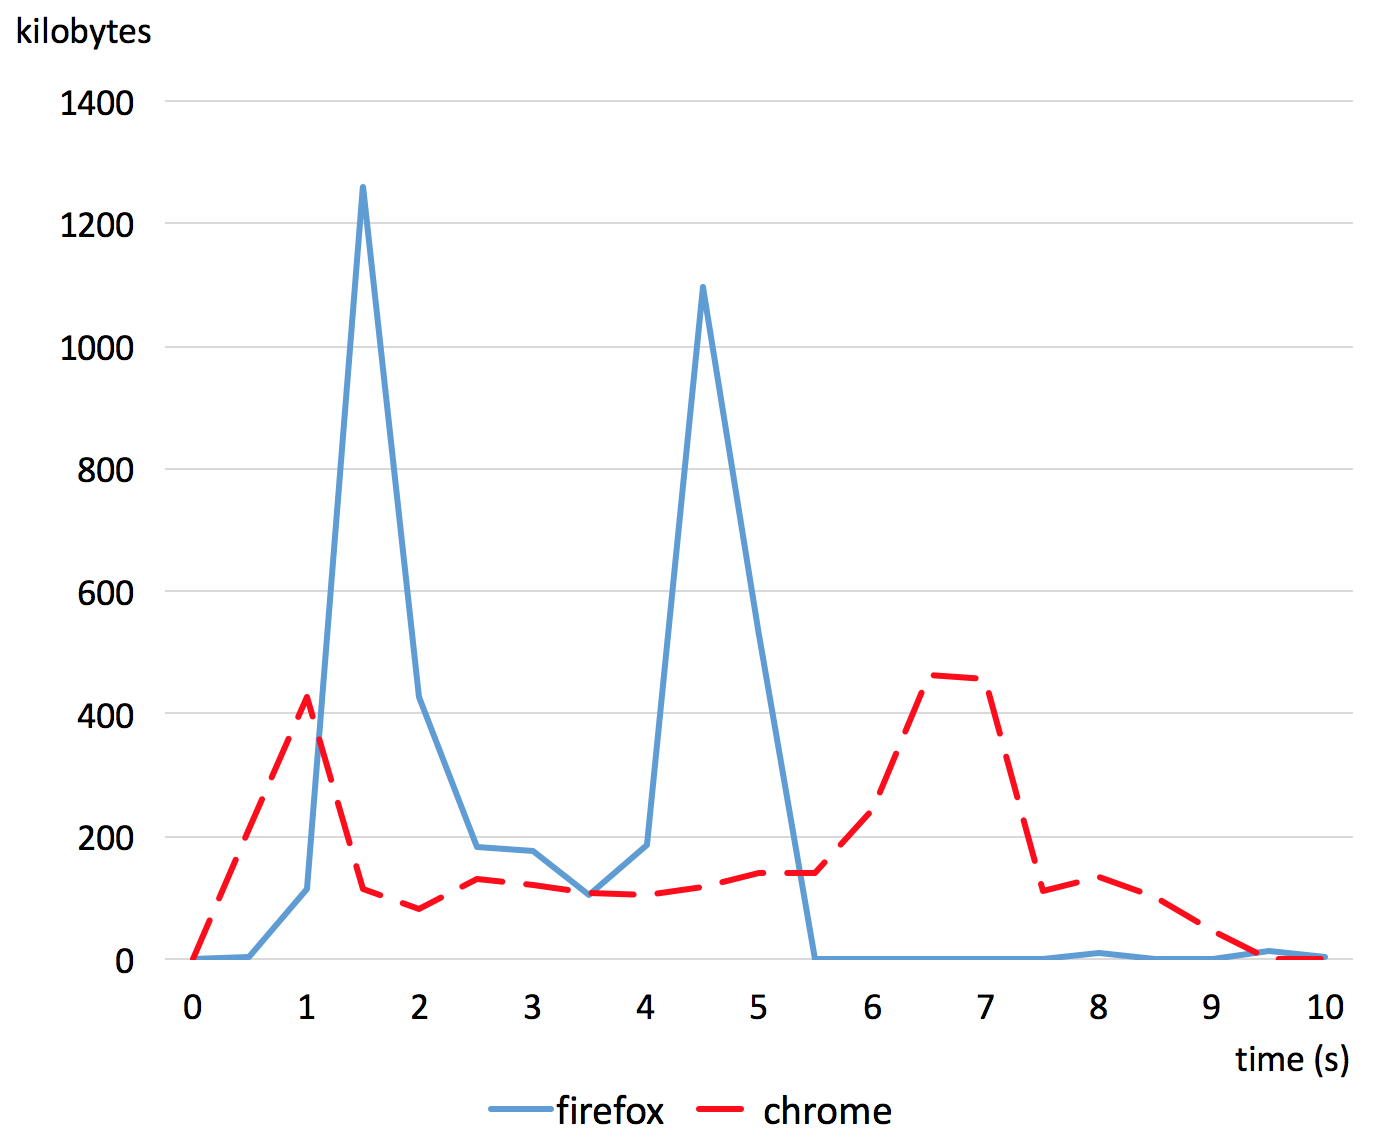
\includegraphics[width=1\columnwidth]{figures/firechrome.png}
\centering
\caption{Comparing link prefetching behavior of Firefox and Chrome for our test webpage\cite{tj-wired}}
\label{fig:firechrome}
\end{figure}



It is our conclusion that it is this deviation of the Tor browser from the expected behavior that causes all of our specified prefetching requests to not be serviced and prevents us from getting the packet capture containing traffic for the prefetching requests and responses.  


%Values &  1800 &    1400  &    2422900    & 455100 

